\section{Introduction}
\label{sec:intro}

When an offline benchmark for microservice root cause analysis (RCA) reports that method $A$ outperforms method $B$, what does the claim apply to?
Benchmarks such as \openrca~\citep{xu2025openrca}, \rcaeval~\citep{pham2024rcaeval}, and \petshop~\citep{hardt2024petshop} each contain several applications or traffic scenarios, which we call subsystems, and methods are ranked by a score pooled over them.
A pooled comparison can be valid for the evaluated mixture without establishing an advantage on each constituent system; yet a method is adopted for one system, and a pooled ranking is read as a guide to that choice.
The number on the leaderboard does not say whether the advantage holds on the system at hand.
It leaves two premises unstated: on which systems the advantage holds, and how the score was produced.
\Cref{fig:teaser} shows one instance of each.
Two pooled leads of similar size (a) differ once split by subsystem (b): one has the same sign on every application, the other is reversed on one scenario with a confidence interval (CI) that excludes zero.
On the same cases, reading the input table that the released runner selects instead of the one its documentation describes (c) reverses a comparison between two published methods, with CIs excluding zero both ways.

\begin{figure}[t]
\centering
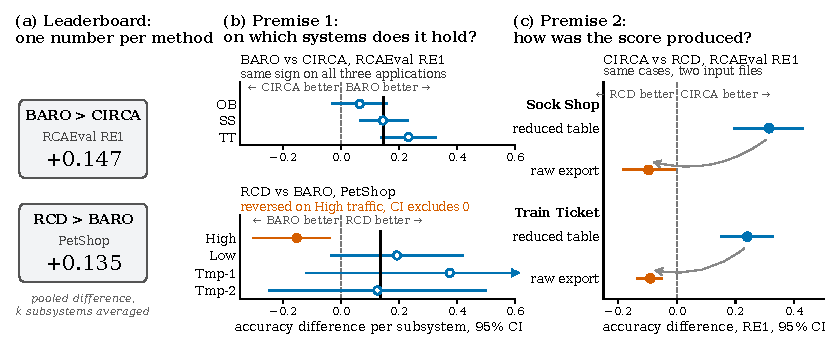
\includegraphics[width=\textwidth]{figures/fig0_teaser.pdf}
\caption{(a) Two pooled comparisons of similar size from two benchmarks. (b) The same comparisons split by subsystem: points are subsystem differences $\Delta_s$ with 95\% bootstrap CIs, the vertical bar is the pooled difference, labels name the method each side favours, and orange marks a subsystem whose sign is opposite to the pooled one, filled when its CI excludes 0. (c) On the same \rcaeval cases, the two input tables that the release ships reverse \circa vs \rcd on two applications, with CIs excluding 0 under both.}
\label{fig:teaser}
\end{figure}

Three observations motivate a systematic check.
First, papers report per-system results but state superiority over the whole benchmark, and the per-case outputs needed to check such a claim with its uncertainty are rarely released.
Second, the releases leave choices to whoever runs them, and some of these choices change scores without raising an error: \rcaeval ships two metric tables per case for two of its applications and its runner reads the one its documentation does not describe; one method returns its input column order under a newer version of a dependency the release does not pin; and a duplicated column header in 50 input tables makes another method fail in the same silent way.
Third, recent work asks whether these benchmarks are hard enough~\citep{fang2025simplerca}, but not which of the comparisons drawn from them hold across their subsystems.

We audit three public benchmark families, 11 subsystems in the main analysis and a second, independently collected release of three of the applications, running the released implementations of 16 methods (10 published methods, 3 simple probes, and 3 baselines shipped by a benchmark) under recorded configurations and scoring them case by case on every case of the subsystems where they run; we compare these runs, not the numbers the original papers report.
We ask one question about each premise.
\textbf{RQ1 (scope):} how stable are comparisons between published methods across the subsystems of a benchmark, and across a second release of the same applications?
\textbf{RQ2 (provenance):} which choices in the released pipeline---the input representation, the handling of failed outputs, the denominator, and the scoring and weighting rule---change these comparisons, and by how much?

Our findings are:
\begin{itemize}
\item \textbf{A pooled lead does not say on which systems it holds.} Of \NMainPubPairs comparisons between published methods, \NMainPubRev reverse on some subsystem, \NMainPubRevCI with CI support, both on one \petshop scenario. Of \NCrossPub comparisons repeated on the second release, \NCrossPubAgree keep their sign and \NCrossPubCIopp have CIs on opposite sides of zero; on Sock Shop, \baro's lead over \circa of \CrossBaroCircaSSOne becomes a deficit of \CrossBaroCircaSSTwo. A ranking computed on all subsystems but one picks the less accurate of two adjacent methods on the held-out subsystem in \HErr of \HNDec decisions. On several subsystems a probe, or a baseline shipped by the benchmark itself, is more accurate than every published method.
\item \textbf{How the score was produced can reverse it.} The input table that the released runner reads reverses \circa against \rcd on two applications, with CIs excluding zero in both directions. Two failures leave no trace on the leaderboard: a method returns its input column order under a drifted dependency, and the duplicated header produces the only CI-supported reversal between published methods on \rcaeval's first release, which disappears once the header is removed. The denominator, the fault composition, and the scoring rule move only differences that are already close to zero.
\item \textbf{Published papers do not release what is needed to check either premise.} Of \SurveyN RCA papers we examined (\cref{sec:bg-survey}), every one that evaluates more than one system reports per-system results, \SurveyRelAny release per-case outputs, each for one method or setting, and none of the \SurveyRelFullCheckable whose releases we could check releases enough to recompute its main paired comparisons without rerunning the methods.
\end{itemize}

This paper contributes:
(i) a matched per-case table over three RCA benchmark families and 16 methods, with the configuration of every run, and two integrity checks for released pipelines that anyone can apply: whether the runner reads the input table that the documentation describes, and whether a method's ranking equals its input column order;
(ii) a quantification of the two unstated premises, the scope of pooled comparisons across subsystems, a second release, and held-out subsystems, and the provenance of scores across four stages of the released pipelines; and
(iii) a reporting format that states both premises, with recommendations to benchmark maintainers tied to the problems we verified.
We do not propose an RCA method.
